Il \textit{Tabu search} é un algoritmo meta euristico di ricerca locale. La differenza principale rispetto all'algoritmo genetico é che, durante la sua esecuzione, tiene traccia delle soluzioni calcolate e non solo dell'ultima trovata. Da questo si può intuire come la memoria e la sua gestione giochi un ruolo chiave in questo tipo di approccio. Ad ogni iterazione, l'algoritmo cerca di trovare la soluzione più conveniente, anche se questa é una mossa peggiorativa rispetto all'ultima soluzione trovata. Il motivo per la quale si accettano soluzioni peggiori è per evitare che l'algorimo si soffermi in un ottimo locale; tuttavia, così facendo, c'è il pericolo che l'algoritmo vada in stallo a causa di cicli: per questo motivo viene introdotta una lista tabu all'interno della quale vengono memorizzate le mosse proibite, ovvero le ultime mosse calcolate. Indicando con $l_t$ la lunghezza della lista tabù, così facendo si evitano cicli di dimensioni $\le l_t$. Quindi nel \textit{tabu search}, l'ultima soluzione trovata dipende dalle soluzioni precedenti e dall'intorno della soluzione stessa.
   
Di seguito verrà esposto come é stata implementata questa strategia per risolvere il problema del \ddbp

\subsection{Algoritmo}
In questa sezione verrà esposto lo pseudocodice utilizzato e verranno spiegate le sue funzionalità. L'algoritmo sviluppato é una piccola variante di quello proposto nei paper \cite{lmvTabu} e \cite{lmvTspack}.

L'algoritmo inizia la sua esecuzione partendo da una soluzione ammissibile del problema: la soluzione ammissibile scelta corrisponde a inserire ciascun pacchetto in un bin diverso, di conseguenza inizialmente il numero di contenitori totale equivale al numero di pacchetti. Successivamente, ad ogni iterazione l'algoritmo cerca di migliorare la soluzione corrente effettuando una mossa migliorativa, cercando tra le soluzioni vicine.

La mossa migliorativa viene scelta secondo il seguente criterio: l'algoritmo deve determinare il bin che é più facilmente svuotabile (\textit{bin target}) e, preso un pacchetto $j$ appartenente al \textit{bin target}, si cerca di aggiungere questo pacchetto all'interno di un insieme di pacchetti $S$: quest'ultimo insieme viene creato prendendo i pacchetti contenuti in $k$ bin, diversi da quello target; per esempio, con $k=1$, l'insieme $S$ é formato dal contenuto di un altro bin e il pacchetto $j$, con $k=2$, l'insieme $S$ é formato dai pacchetti presenti in due bin più il pacchetto $j$, e così via.

Il \textit{target bin} é il bin che si presume sia più facile da svuotare; dato un insieme di bin, questo bin é quello che minimizza il risultato della seguente funzione (\textit{filling function}):
\[
   \varphi(S_i) = \alpha\frac{\sum_{j\in S_i}w_jh_j}{WH}-\frac{|S_i|}{n}
\]
dove:
\begin{itemize}[noitemsep]
   \item $S_i$ = insieme di pacchetti presenti nell'$i-$esimo bin;
   \item $\alpha$ = parametro di configurazione;
   \item $w_j$ = larghezza pacchetto $j-$esimo;
   \item $h_j$ = altezza pacchetto $j-$esimo;
   \item $|S_i|$ = \# pacchetti presenti nell'$i-$esimo bin;
   \item $n$ = \# pacchetti totali del problema;
\end{itemize}
Oltre alla scelta del \textit{target bin}, é necessario porre attenzione anche al valore di $k$ per i seguenti motivi:
\begin{enumerate}[noitemsep]
\item indica la dimensione delle soluzioni vicine su cui cercare;
\item influisce sulla velocità di esecuzione dell'algoritmo; infatti, indicando con $B$ l'insieme di bin, i $k$ bin possono essere presi in $\binom{|B|-1}{k}$ modi (viene escluso dai possibili bin il \textit{bin target});
\end{enumerate}

Questo é lo pseudocodice dell'algoritmo utilizzato:
\texttt{\footnotesize
   \begin{tabbing}
   \=~~~\=~~~\=~~~\=~~~\\
   Algoritmo TABU($k_{max},d_{max}$,dimensioni liste tabu)\\\\
   inizializza ciascuna lista tabù a vuoto\\
   inserisci ciascun pacchetto in un bin\\
   $z=n, d=1$\\
   determina target bin $t$\\
   while (not(condizione di stop)) do\\
   \>\>diversify=false; $k=1$\\
   \>\>while (diversify==false) do\\
   \>\>\>$k_{in}$ = $k$\\
   \>\>\>SEARCH($t,k,$diversify,$z$)\\
   \>\>\>$z^* = $min($z, z^*$)\\
   \>\>\>if ($k < k_{in}$) then\\
   \>\>\>\>trova il nuovo target bin $t$\\
   \>\>end while\\
   \>\>DIVERSIFICATION($d,z,t$)\\
   end while\\\\
   end\\
   \end{tabbing}
}

In input l'algoritmo richiede i seguenti valori:
\begin{itemize}[noitemsep]
\item $k_{max}$: dimensione massima per $k$;
\item $d_{max}$: dimensione massima per $d$;
\item dimensioni liste tabu: specifica la lunghezza massima di ciascuna lista tabu ($k=1, k>1$);
\end{itemize}

L'algoritmo di placing utilizzato per posizionare i pacchetti all'interno del bin, indicato con \texttt{A(\{1,...,n\})}, é naturalmente il BLF (Bottom Left Fill).

Il \textit{Tabu Search} é composto principalmente da due metodi, \texttt{SEARCH} e \texttt{DIVERSIFICATION}, la cui implementazione é spiegata di seguito.

\subsubsection{SEARCH}
L'obiettivo principale di questo metodo é quello di visitare le soluzioni vicine a quella corrente, rimuovendo un pacchetto $j$ presente nel \textit{target bin} e inserendolo in un altro bin. Il numero di soluzioni che verranno analizzate dipendono ovviamente dal parametro di input $k$.

Il funzionamento di questo metodo segue questi passi:
\begin{enumerate}[noitemsep]
   \item per ciascun pacchetto presente nel \textit{target bin}, viene selezionato un possibile sottoinsieme $U$ di bin di cardinalità $k$ fra quelli presenti nella soluzione attuale (\textit{target bin} escluso)
   \item viene creato l'insieme $S$ di pacchetti inserendo il pacchetto $j-$esimo con tutti i pacchetti presenti nei bin dell'insieme $U$;\\$S = \{j\} \cup (\bigcup_{i\in U}S_i)$;
   \item si chiama all'esecuzione l'algoritmo di placing BLF sull'insieme S;
   \item in base alla soluzione trovata dal BLF, si decide se ritornare la soluzione o riprovare con un altro pacchetto;
\end{enumerate}

Di seguito viene riportato lo pseudocodice:
\texttt{\footnotesize
   \begin{tabbing}
   ~~~\=~~~\=~~~\=~~~\=~~~\=~~~\\
   SEARCH($t,k$,diversify,$z$)\\\\
   penalty$^* = +\infty$\\
   for each $j \in S_t$ do\\
   \>for each insieme $U$ di bins escluso quello target t do\\
   \>\> $S = \{j\} \cup (\bigcup_{i\in U}S_i)$\\
   \>\> penalty = $+\infty$\\
   \>\> case\\
   \>\>\> A(S) < k\\
   \>\>\>\> esegui la mossa\\
   \>\>\>\> $k = $max$\{1, k-1\}$\\
   \>\>\>\> return\\
   \>\>\> A(S) = k\\
   \>\>\>\> if (mossa non in lista tabu) o ($S_t \equiv \{j\}$) then\\
   \>\>\>\>\> esegui la mossa\\
   \>\>\>\>\> if $S_t \equiv \{ j\}$ then $k = $max$\{1, k-1\}$;\\
   \>\>\>\>\>return\\
   \>\>\>\>endif\\
   \>\>\> A(S) = k+1 e k>1\\
   \>\>\>\> I = insieme di k+1 bin usati da A\\
   \>\>\>\> $t'$ = argmin$_{i\in I}\{\varphi(S_i)\}$\\
   \>\>\>\> $T = (S_t \backslash \{j\})\cup S_{t'}$\\
   \>\>\>\> if (A(T)==1) e (mossa non in lista tabu) then\\
   \>\>\>\>\> penalty = min$\{\varphi(T),$ min$_{i\in I \backslash t'}\{\varphi(S_i)\}\}$\\
   \>\>end case\\
   \>\> penalty$^*$ = min$\{$penalty$^*$, penalty$\}$\\
   \> end for\\
   end for\\\\
   if (penalty$^* \ne +\infty$) then\\
   \> esegui la mossa corrispondente a penalty$^*$\\
   else\\
   \> if ($k = k_{max}$) then\\
   \>\> diversify = true\\
   \> else\\
   \>\> $k = k+1$\\
   return
   \end{tabbing}
}

Come si può notare dall'algoritmo, ci possono essere tre situazioni diverse a seconda del risultato ottenuto dalla chiamata del BLF sull'insieme $S$ (con \texttt{A(S)} viene indicato il numero di bin utilizzati per impacchettare i pacchetti presenti nell'insieme $S$):
\begin{enumerate}[noitemsep]
   \item \texttt{A(S) < k}: in questo caso, il pacchetto $j$ viene rimosso dal target bin e il numero di bin prodotti per inserire tutti i pacchetti presi in esame é minore del numero di bin presi per costruire $S$. Qual'ora il target bin sia composto dal solo pacchetto $j$, avviene l'eliminazione anche del target bin. La soluzione ottenuta é migliore di quella attuale;
   \item \texttt{A(S) = k}: anche in questo frangente il pacchetto $j$ viene rimosso dal target bin ma la quantità di bin utilizzati per $S$ non é cambiato. Anche in questo caso, se il target bin é composto dal solo pacchetto $j$, si procede con la sua eliminazione. La soluzione ottenuta é migliore di quella attuale se é stato eliminato il bin target, altrimenti é equivalente.
   \item \texttt{A(S) > k}: in quest'ultimo caso viene trovata una soluzione peggiore di quella attuale.
\end{enumerate}

Nei primi due casi, essendo la soluzione migliorativa o equivalente a quella attuale, la soluzione trovata é restituita al tabu search. Se la nuova soluzione é migliore, il parametro $k$ viene diminuito.

Nell'ultimo caso la soluzione trovata é peggiore: per evitare che successivamente venga effettuata questa mossa, viene calcolata una \textit{penalty} che verrà associata alla nuova soluzione.

A seconda della soluzione trovata, questa funzione salva una \textit{descrizione della soluzione} nella \textit{tabu list}; come scelta implementativa, esiste una \textit{tabu list} per ogni valore di $k$, di conseguenza si avranno al più $k_{max}$ liste tabu. Esse sono riempite con questa modalità:
\begin{itemize}[noitemsep]
   \item \textit{$k=1$}: viene inserito il valore della \textit{filling function} $\varphi(S)$ dell'ìnsieme $S$ per la quale é stata trovata una soluzione;
   \item \textit{$k>1$}: nella lista tabu $k-$esima, viene inserita la \textit{penalty} associata alla soluzione peggiorativa trovata;
\end{itemize}

La scelta di memorizzare nelle liste tabu questi valori é atta a migliorare le prestazioni dell'algoritmo tabu; la scelta peggiore sarebbe stata quella di salvare nelle liste, per ogni mossa, l'insieme di pacchetti della soluzione trovata. Ovviamente questo ha un impatto negativo sulle prestazioni, in quanto per verificare se una mossa é presente o meno nella lista tabu, sarebbe stato necessario scorrere tutti i pacchetti.
\subsubsection{DIVERSIFICATION}
Questo metodo viene chiamato qual'ora l'ultima soluzione trovata sia stata peggiorativa e la cui penalty associata fosse uguale a $\infty$.

Ci sono due tipi di diversificazione:
\begin{enumerate}[noitemsep]
   \item conservativa: in questo caso, viene scelto un nuovo target bin; più precisamente, viene selezionato il bin con il $d-$esimo valore più piccolo della filling function;
   \item non conservativa: dalla soluzione corrente, posto $z = \#$ bin della soluzione corrente, vengono presi i $\big\lfloor \frac{z}{2} \big\rfloor$ con valore della filling function minore e, per ciascun pacchetto presente in questi bin, viene creato un nuovo contenitore.
\end{enumerate}

Questo é lo pseudocodice:
\texttt{\footnotesize
   \begin{tabbing}
   ~~~\=~~~\=~~~\\
   DIVERSIFICATION($d,z,t$)\\\\
   if ($d \le z$) e ($d < d_{max}$) then\\
   \>$d = d+1$\\
   \>$t$ = target bin con il d-esimo valore più piccolo della funzione $\varphi(\cdot)$\\
   else\\
   \>prendi i $\big\lfloor \frac{z}{2} \big\rfloor$ contenitori con valore della $\varphi(\cdot)$ minore e, \\
   \>per ciascun pacchetto in essi, crea un nuovo contenitore\\
   \>$d=1$\\
   return
   \end{tabbing}
}

\subsection{Inconveniente}
Seguendo l'approccio menzionato dai paper precedenti, durante lo sviluppo del nostro algoritmo tabu é apparso un inconveniente, derivante dall'utilizzo del \textit{BLF} come algoritmo di placing.

Nella procedura \texttt{SEARCH}, qual'ora \texttt{A(S)} risultasse pari a $k$, significa che un pacchetto é stato rimosso dal target bin ed é stato aggiunto ad un altro contenitore. Questo porterebbe a dire che i pacchetti presenti nel target bin, essendo in numero inferiore rispetto a prima, possono nuovamente essere riposizionati all'interno del loro contenitore. Il problema é collegato a questo punto: vediamo con un esempio:

Consideriamo la seguente istanza del problema:
\begin{itemize}[noitemsep]
   \item Bin: \textsc{Larghezza = 4} - \textsc{Altezza = 4}
   \item Pacchetti: vedere tabella \ref{table:packets}
\end{itemize}
\begin{table}[htp]
  \small\centering
  \begin{tabular}{c|ccc}
    \toprule
    \textsc{Pacchetto} & \textsc{Larghezza} & \textsc{Altezza} & \textsc{Quantità}\\
    \midrule
    0 & 2 & 1 & 1\\
    1 & 3 & 1 & 1\\
    2 & 1 & 4 & 1\\
    3 & 3 & 1 & 1\\
    \bottomrule
  \end{tabular}
  \caption{Configurazione Pacchetti}
  \label{table:packets}
\end{table}

Applicando l'algoritmo BLF, si ottiene il packing di figura \ref{img:inconv1}:

\begin{figure}[h!]
  \centering
  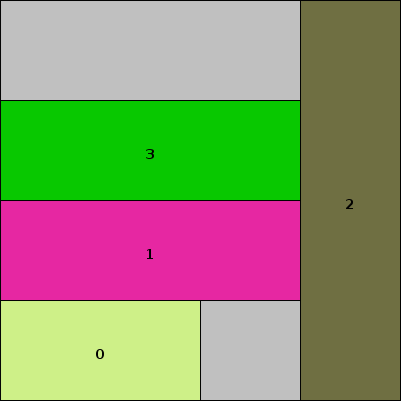
\includegraphics[height=0.3\textwidth]{./img/inconv1.png}
  \caption{BLF: packing 1}
  \label{img:inconv1}
\end{figure}

Ora, supponiamo che la procedura \texttt{SEARCH} rimuova il pacchetto $j=1$ dal contenitore; applicando il BLF ai pacchetti residui, si ottiene il risultato di figura \ref{img:inconv2}:

\begin{figure}[htb]
  \centering
  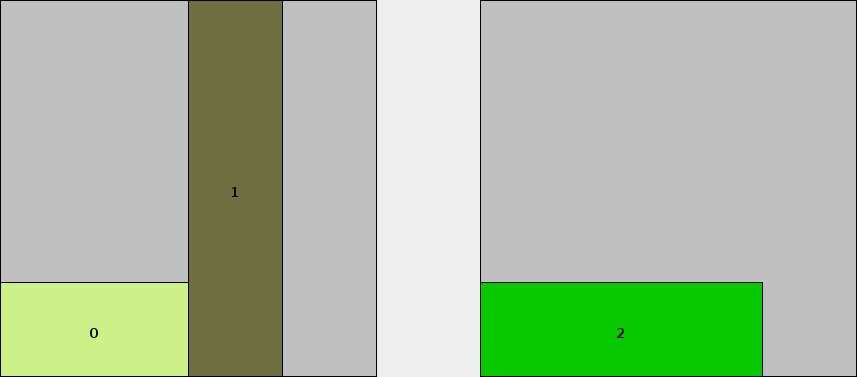
\includegraphics[height=0.3\textwidth]{./img/inconv2.png}
  \caption{BLF: packing 2}
  \label{img:inconv2}
\end{figure}

Come si può notare dall'immagine di figura \ref{img:inconv2}, nonostante sia stato eliminato un pacchetto dal target, il BLF ha richiesto un nuovo contenitore per collocare tutti i pacchetti residui. Questo problema deriva dal fatto che in input il BLF vuole una lista di pacchetti, il cui \textit{ordine} é importante al fine della loro allocazione all'interno del bin.

Dopo diversi test con istanze di problema comuni, é stato scelto che, qual'ora si verificasse questo inconveniente, il programma termini la ricerca dell'ottima avvisando l'utente del motivo dell'interruzione. L'alternativa sarebbe stata quella di trovare una lista di pacchetti tale per cui il BLF ritornasse un solo contenitore con un posizionamento ottimo dei pacchetti: il motivo per la quale questa scelta é stata scartata, deriva dalla possibile durata nel cercare tale lista; infatti, oltre a considerare l'ordine dei pacchetti all'interno della lista, bisogna valutare la possibilità che ciascun pacchetto può essere o meno ruotato. Di conseguenza, indicando con $n = \#$ pacchetti presenti in un bin, le possibili liste sono pari a $\binom{2n}{n}!$ e, essendo la complessità temporale del BLF $O(n^2)$, la complessità per trovare la lista migliore sarebbe stata $O\left((\binom{2n}{n}!)^2\right)$, almeno utilizzando un approccio del tipo \textit{brute force}.

\subsection{Miglioramento per il BLF}
Al fine di migliorare le soluzioni trovate dal tabu search in combinazione con l'algoritmo di placing BLF, é stata introdotta una semplice miglioria: durante la creazione dell'insieme $S$, i pacchetti vengono ordinati per larghezza in modo decrescente: l'introduzione di questa funzionalità deriva dall'idea che un pacchetto grande é più difficile da spostare rispetto ad un pacchetto piccolo.

Svolgendo prove ripetute su diverse istanze del problema, abbiamo verificato come i risultati ottenuti con questa opzione attiva siano migliori rispetto a quelli senza e, per qualche particolare configurazione, é stato raggiunte addirittura l'ottimo.
